\appendix

\section{
    Appendix A
    \\
    \large{Potential Surface Graphs for Squat, Bench, and Deadlift}
}
\label{sec:AppendixA}

\begin{table}[h]
    \centering
    \begin{tabular}{c|c}
        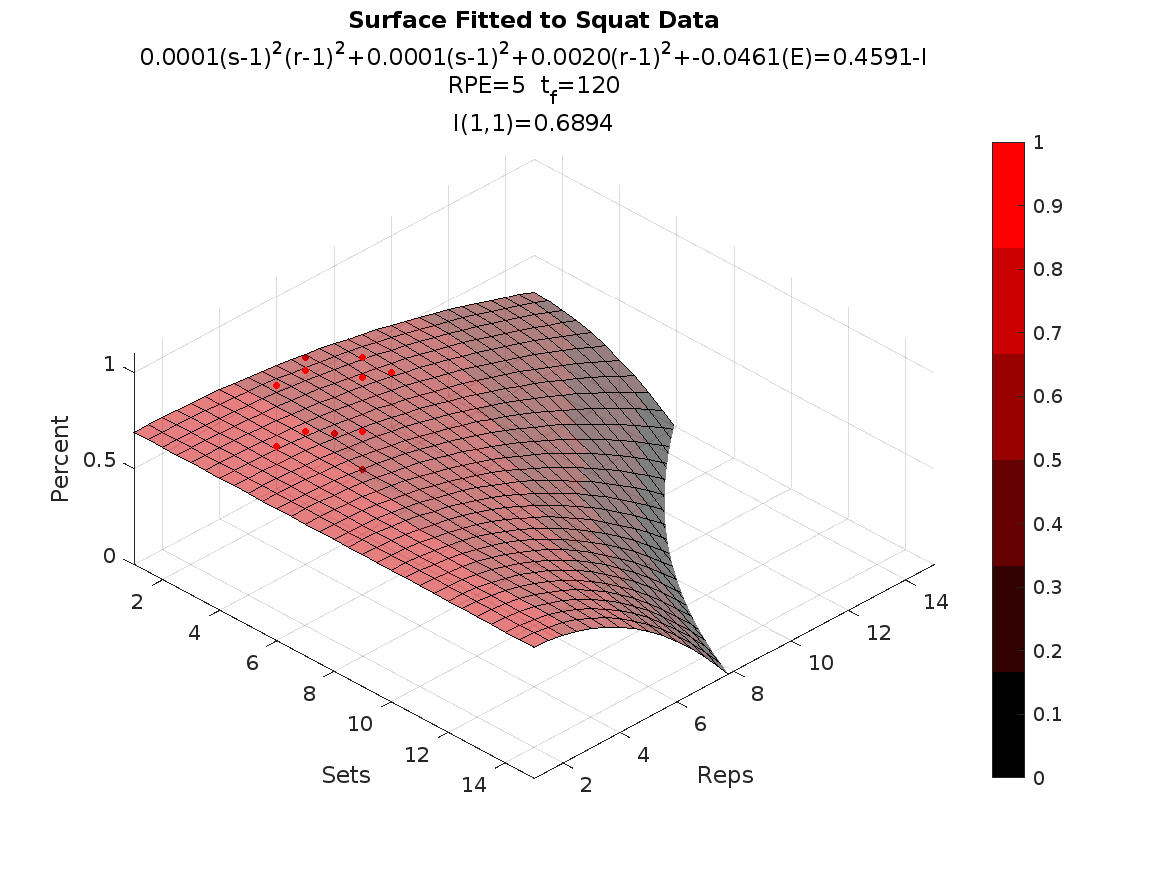
\includegraphics[width=78mm]{SquatSurface/5.png} &  
        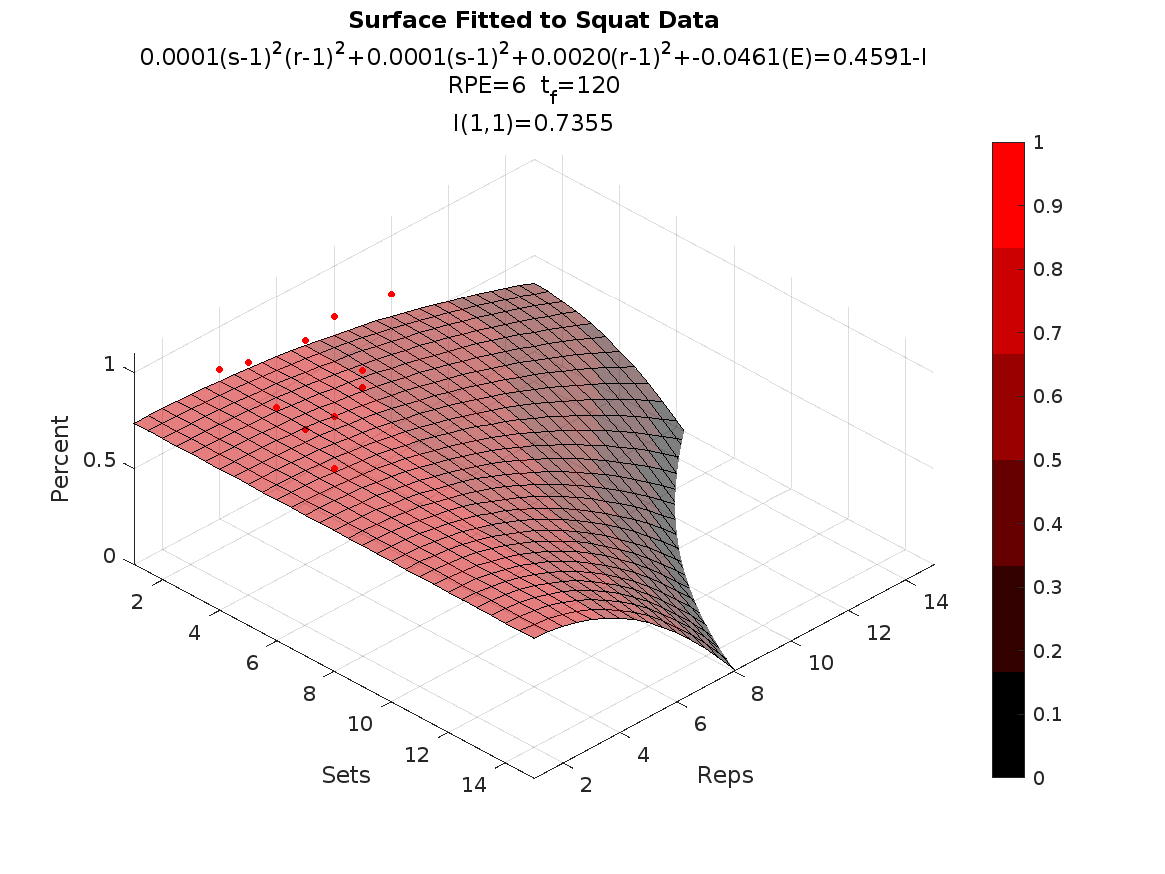
\includegraphics[width=78mm]{SquatSurface/6.png} \\
         
        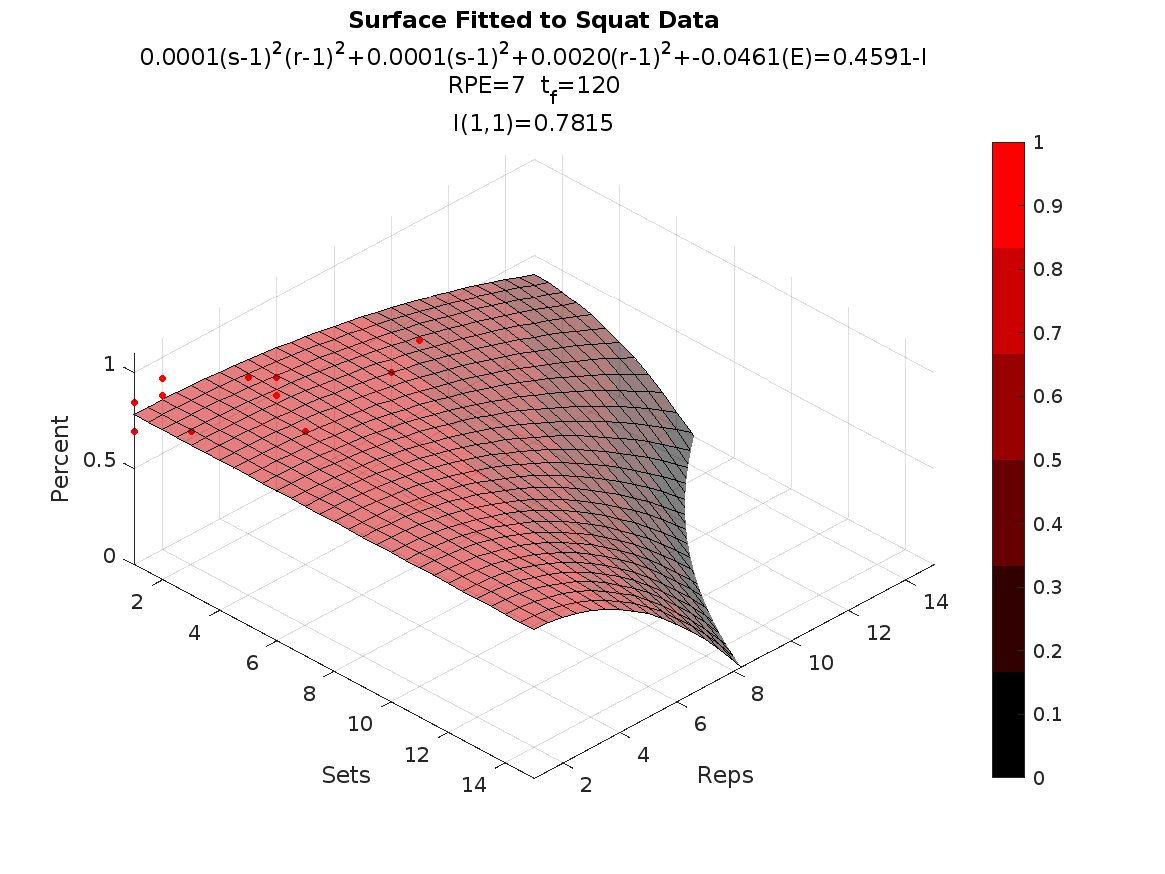
\includegraphics[width=78mm]{SquatSurface/7.png} &
        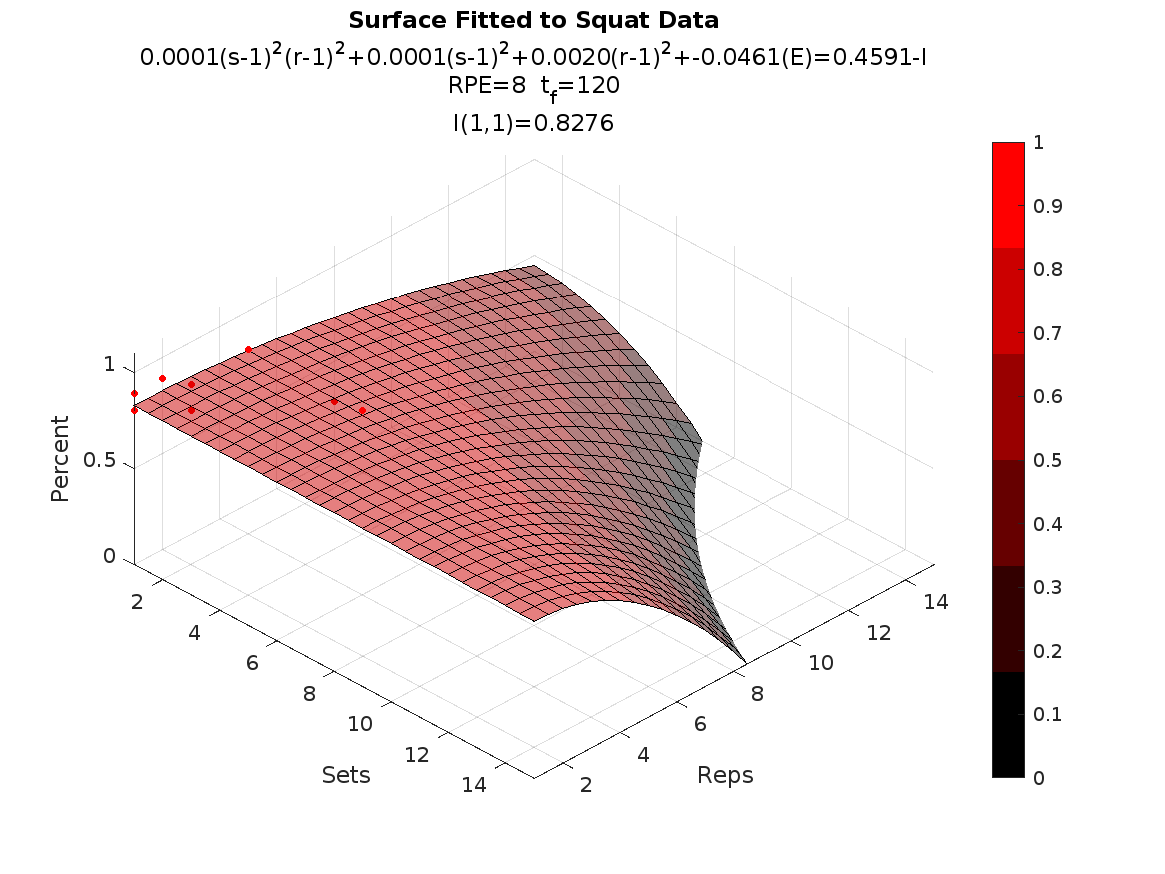
\includegraphics[width=78mm]{SquatSurface/8.png} \\
        
        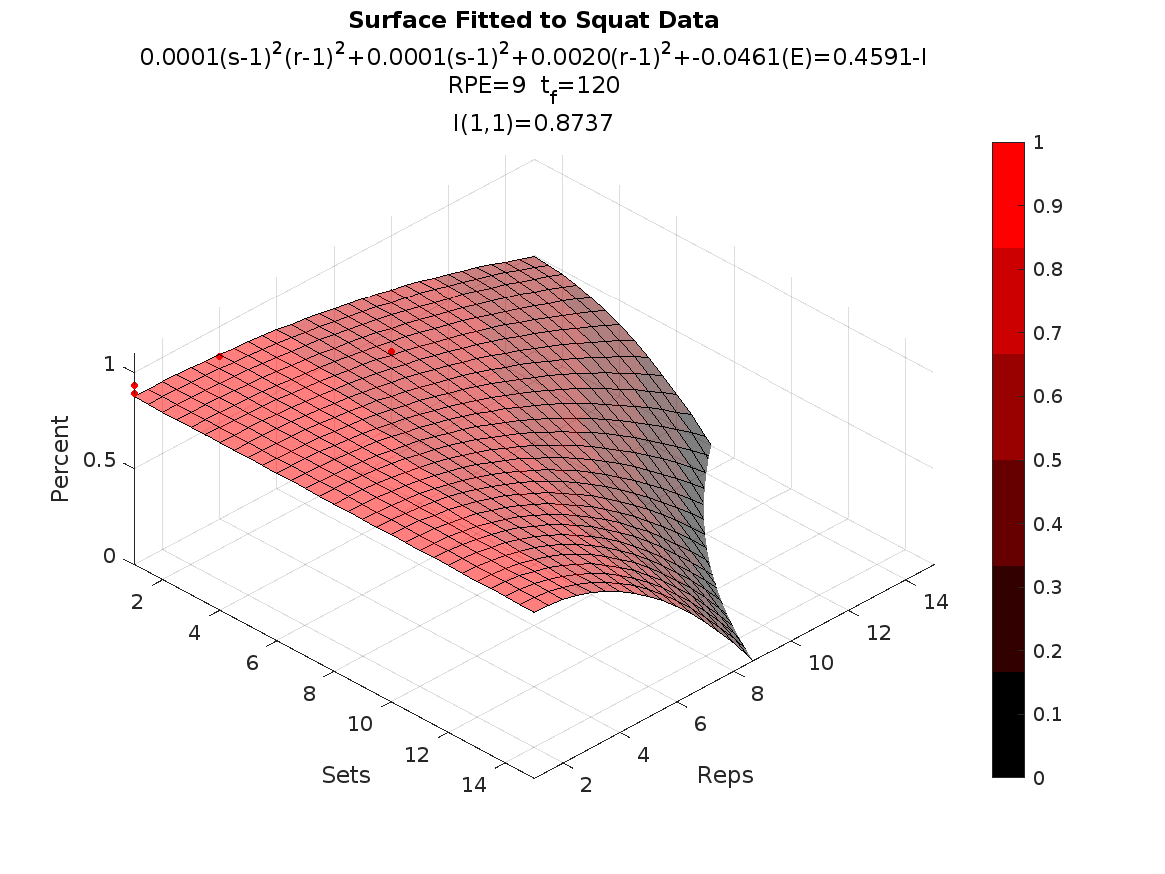
\includegraphics[width=78mm]{SquatSurface/9.png} &
        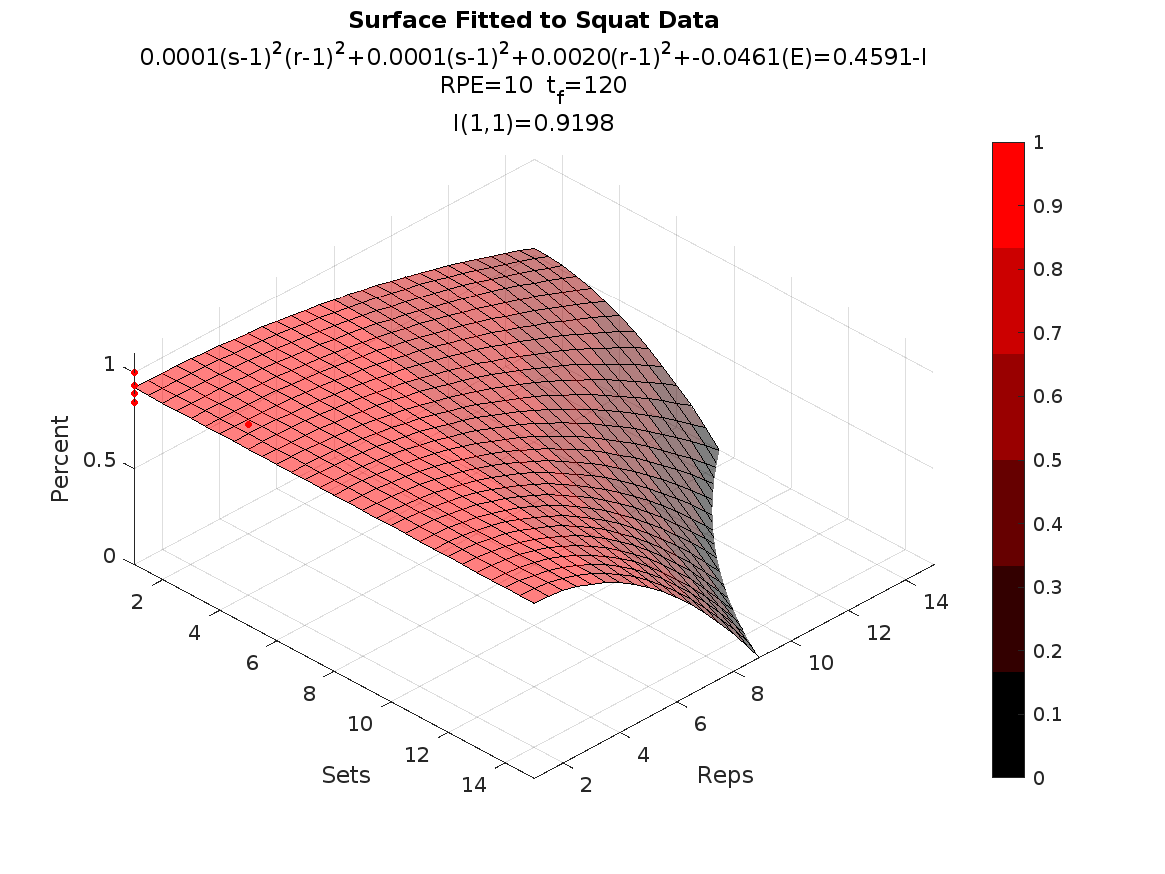
\includegraphics[width=78mm]{SquatSurface/10.png} \\
    \end{tabular}
    \caption{The potential surface fitted to squat data at various effort levels.}
    \label{tab:AppBSquatPotentialSurfaceAcrossEffort}
\end{table}

\begin{table}[h]
    \centering
    \begin{tabular}{c|c}
        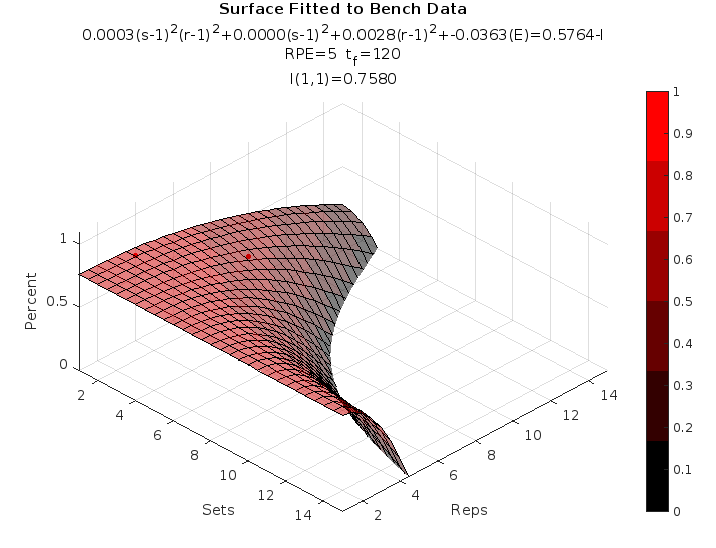
\includegraphics[width=80mm]{BenchSurface/5.png} &  
        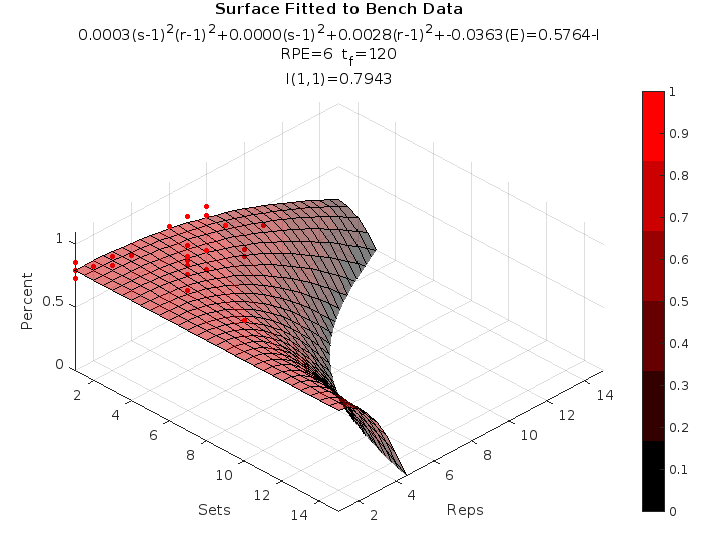
\includegraphics[width=80mm]{BenchSurface/6.png} \\
         
        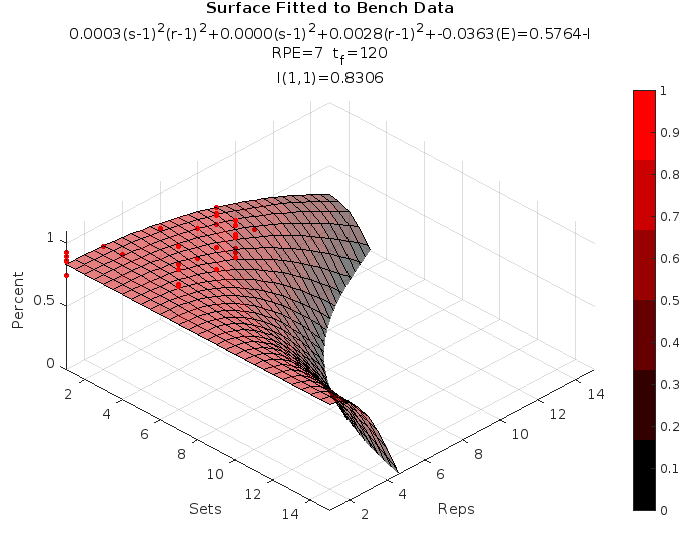
\includegraphics[width=80mm]{BenchSurface/7.png} &
        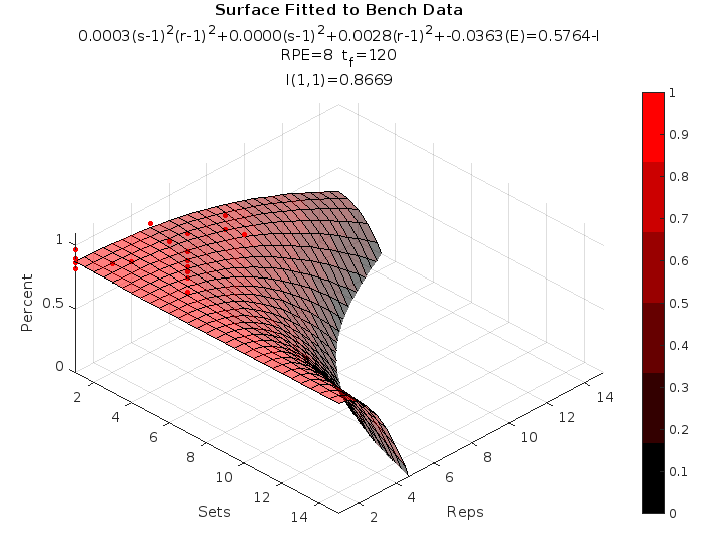
\includegraphics[width=80mm]{BenchSurface/8.png} \\
        
        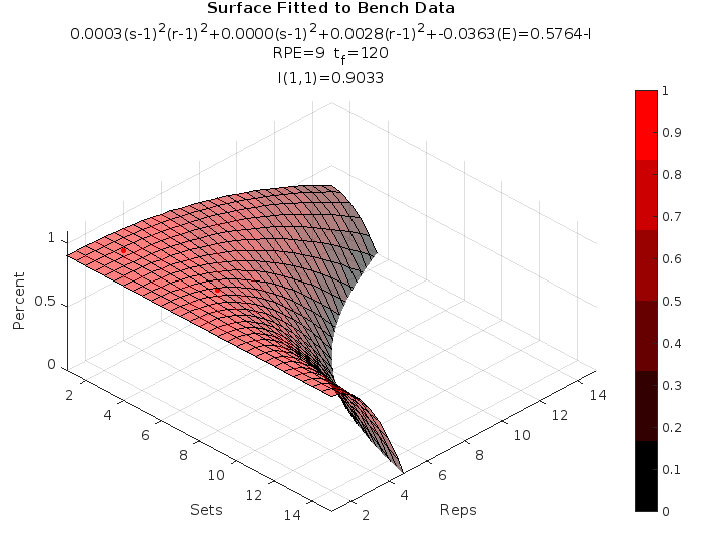
\includegraphics[width=80mm]{BenchSurface/9.png} &
        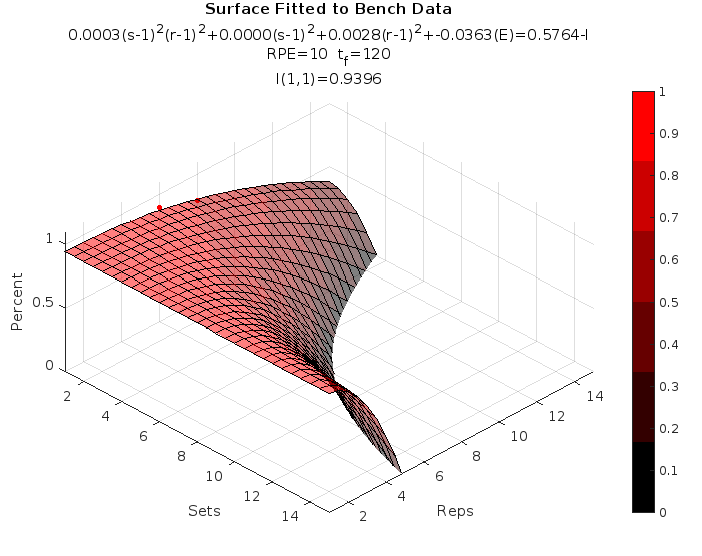
\includegraphics[width=80mm]{BenchSurface/10.png} \\
    \end{tabular}
    \caption{The potential surface fitted to bench data at various effort levels.}
    \label{tab:AppBBenchPotentialSurfaceAcrossEffort}
\end{table}

\begin{table}[h]
    \centering
    \begin{tabular}{c|c}
        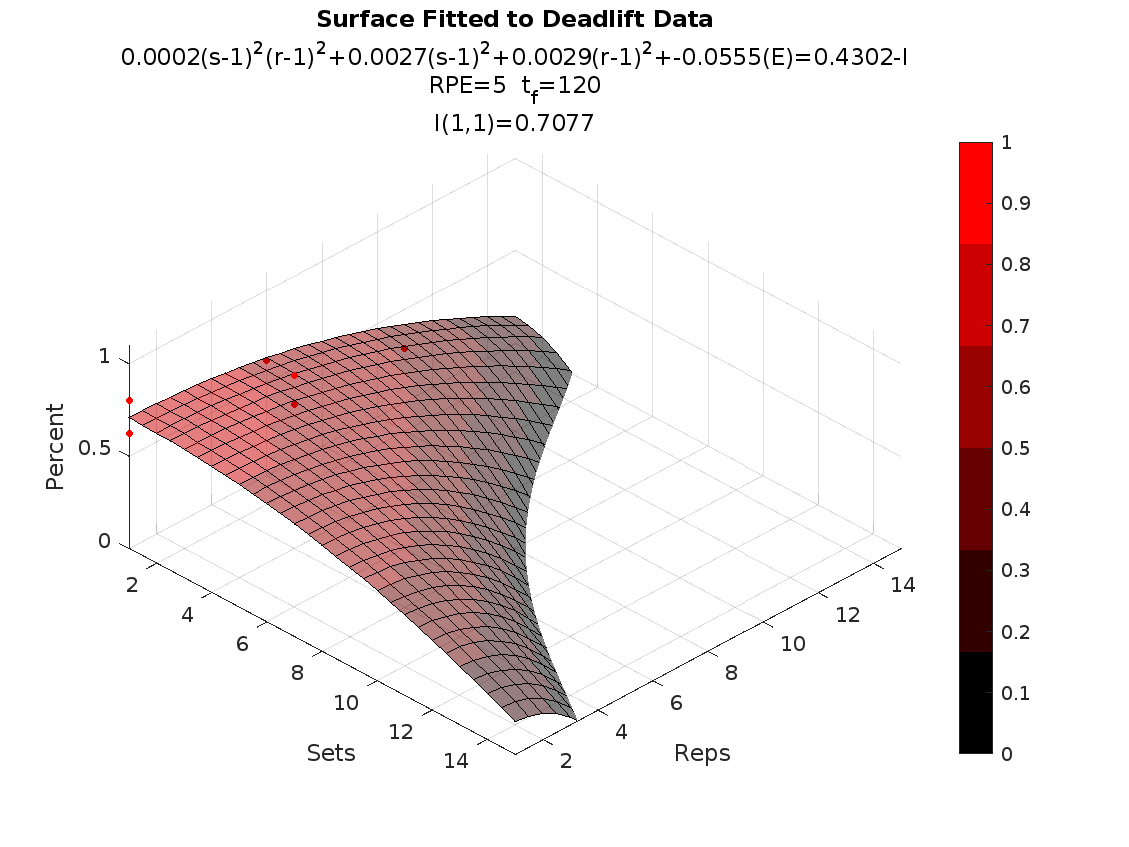
\includegraphics[width=80mm]{DeadliftSurface/5.png} &  
        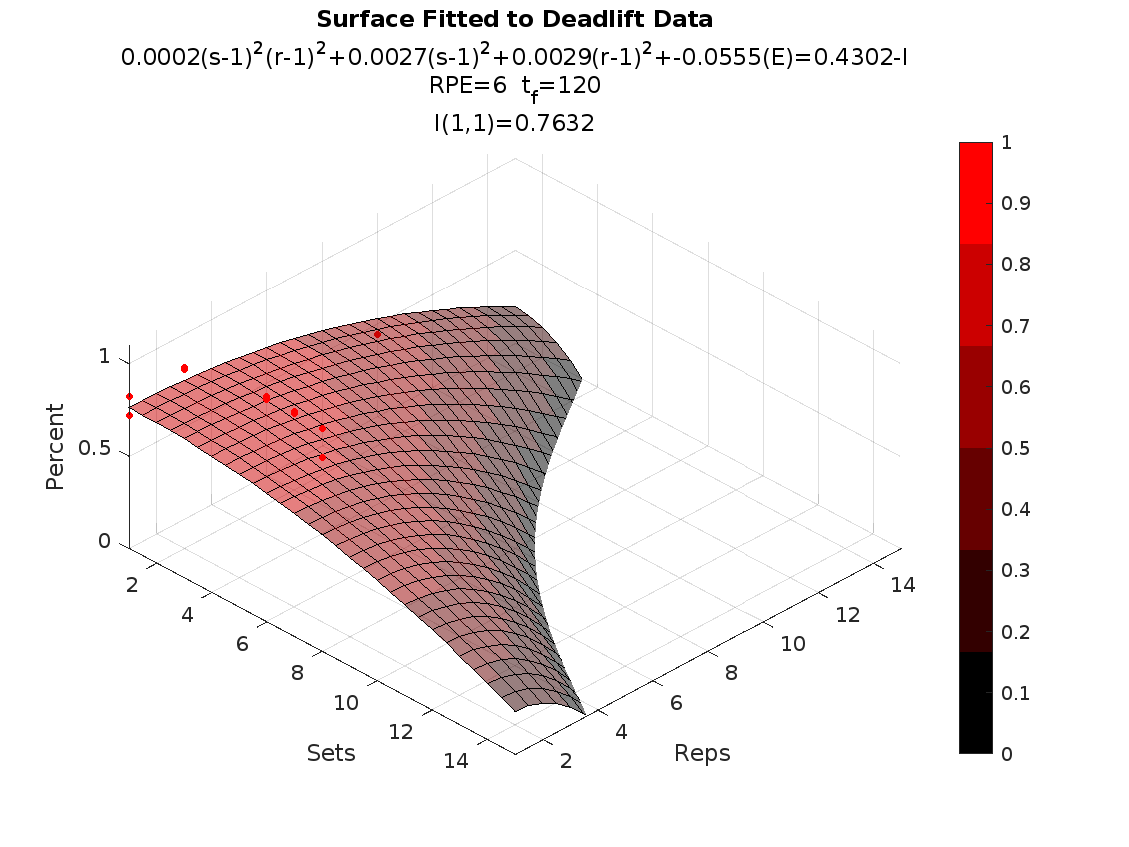
\includegraphics[width=80mm]{DeadliftSurface/6.png} \\
         
        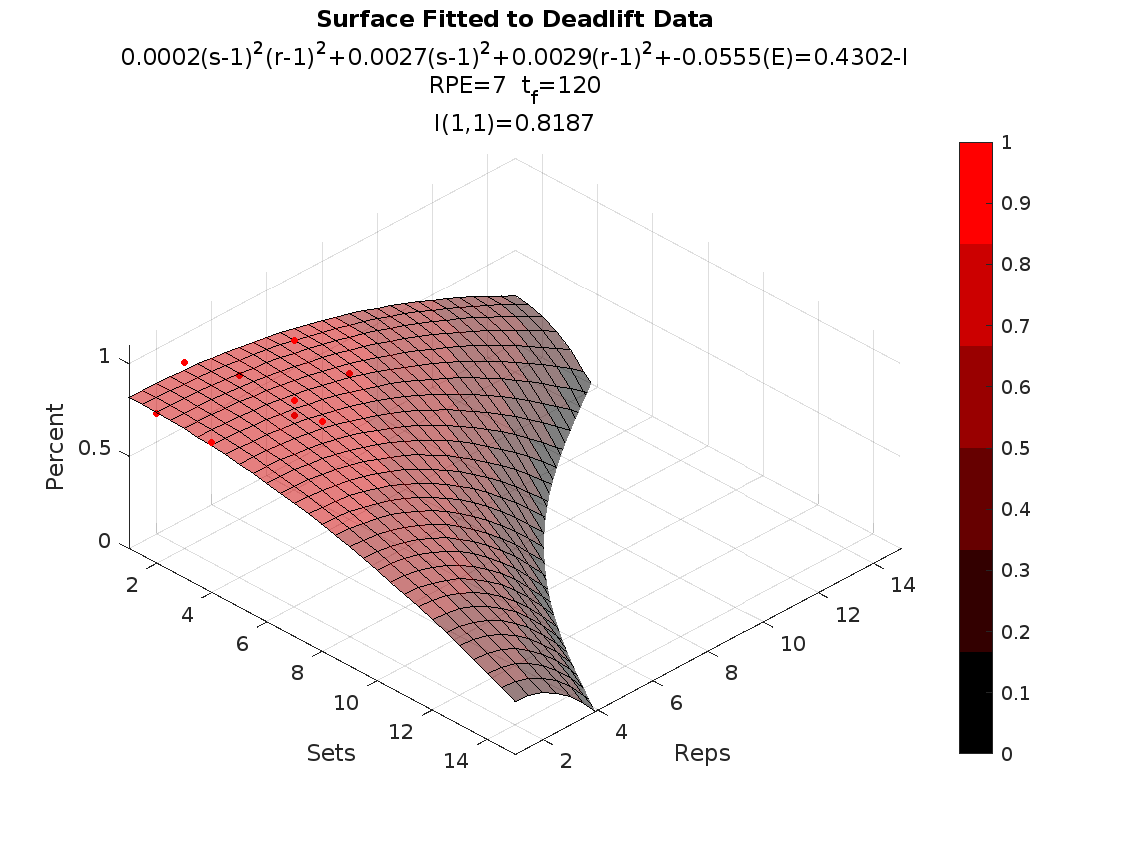
\includegraphics[width=80mm]{DeadliftSurface/7.png} &
        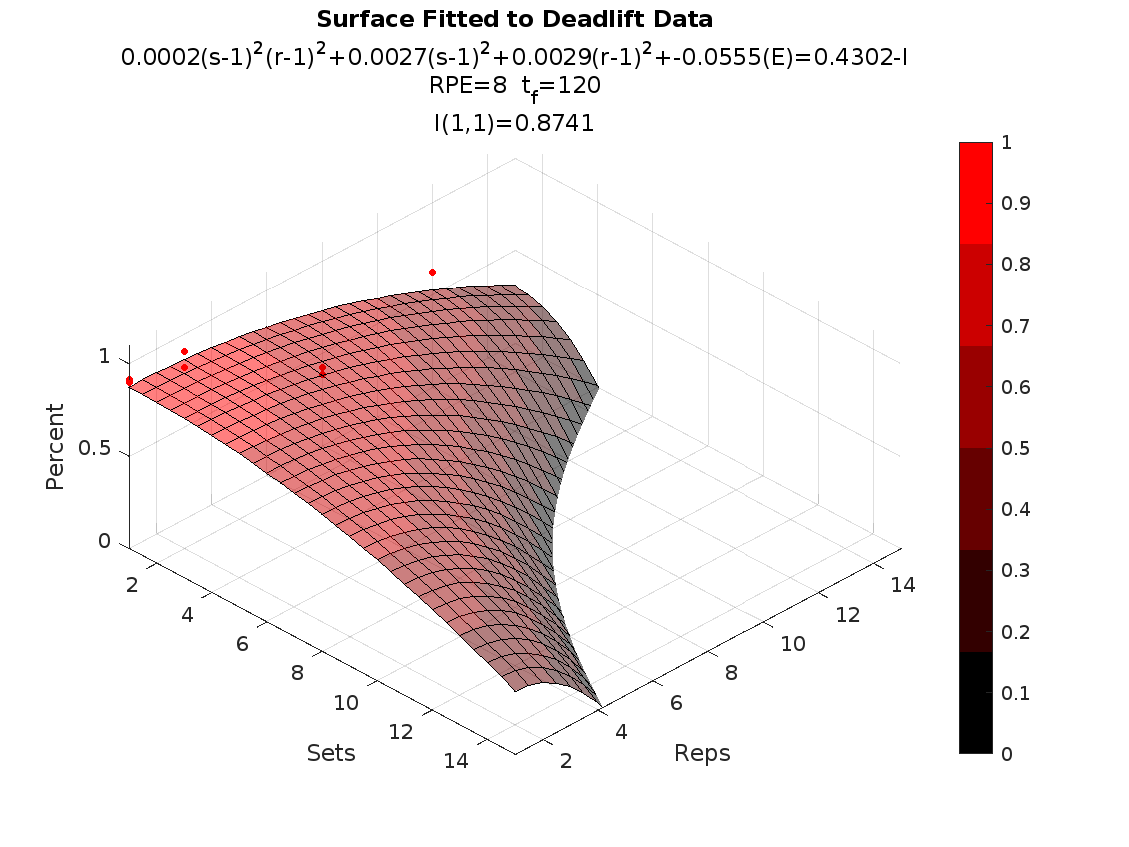
\includegraphics[width=80mm]{DeadliftSurface/8.png} \\
        
        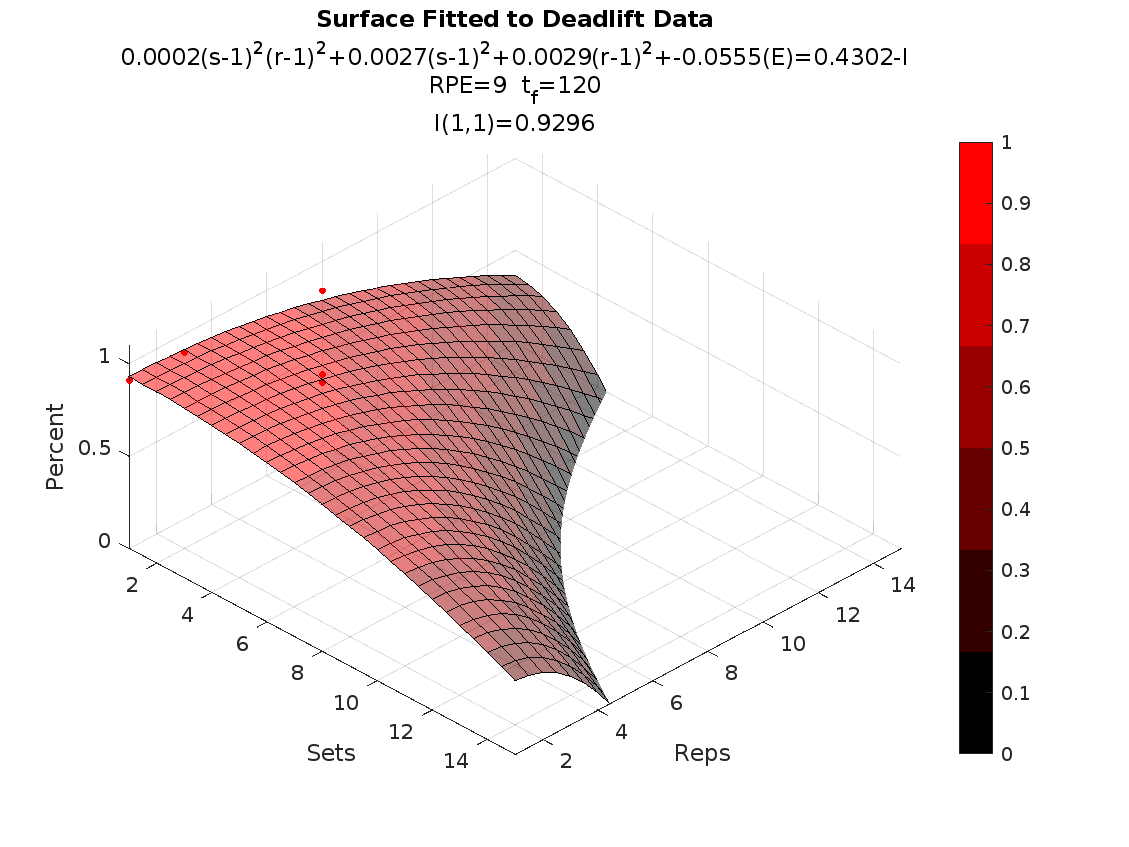
\includegraphics[width=80mm]{DeadliftSurface/9.png} &
        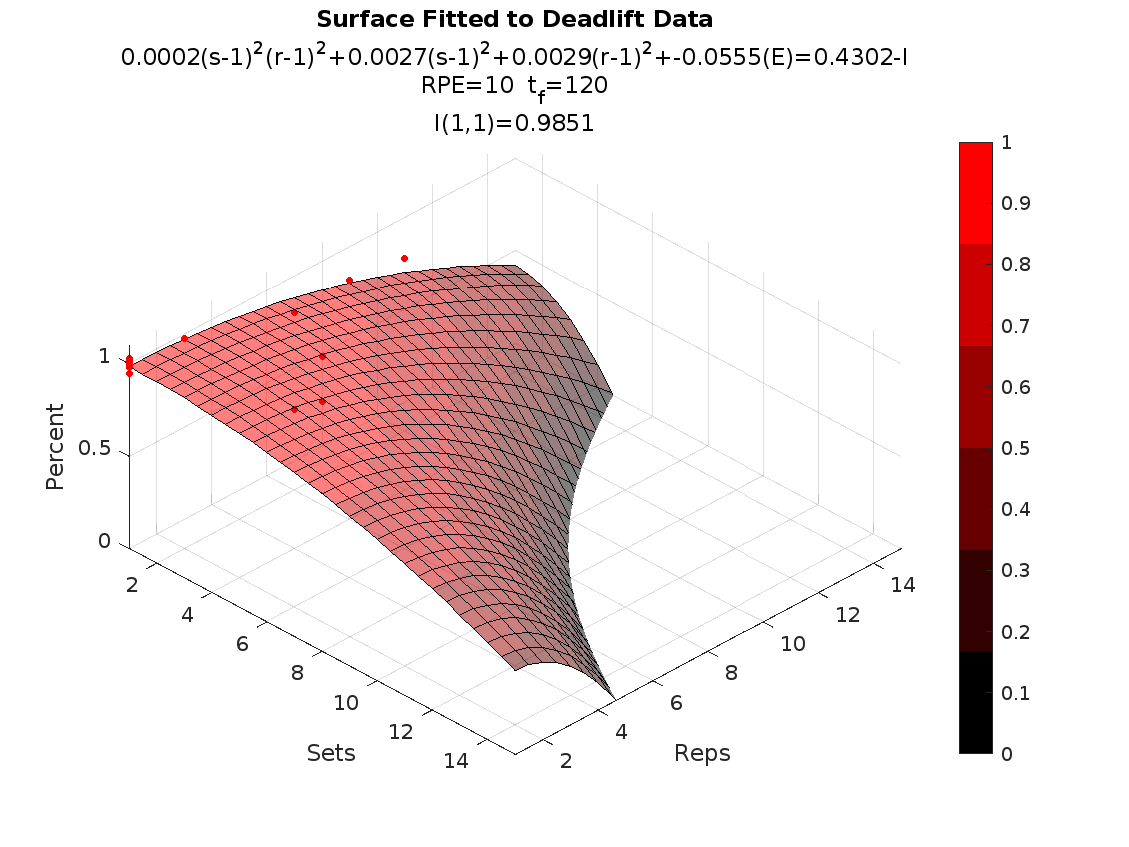
\includegraphics[width=80mm]{DeadliftSurface/10.png} \\
    \end{tabular}
    \caption{The potential surface fitted to deadlift data at various effort levels.}
    \label{tab:AppBDeadliftPotentialSurfaceAcrossEffort}
\end{table}